Un ensayo de filtración por gravedad comienza con \(1\,\mathrm L\) de suspensión homogénea sobre un filtro limpio. Sea \(V\) el volumen de líquido que queda en el depósito y \(m\) la masa de sólido depositada en el filtro. Se adoptan estas leyes idealizadas, con constantes sintéticas:
\[
\Delta p=\left(1\,\frac{\mathrm{kPa}}{\mathrm L}\right)V,
\qquad R=R_0+\beta m,
\qquad Q=\frac{\Delta p}{R},
\]
\[
R_0=1\,\frac{\mathrm{kPa}\,\mathrm{min}}{\mathrm L},
\qquad \beta=1\,\frac{\mathrm{kPa}\,\mathrm{min}}{\mathrm L\,\mathrm g}.
\]
Aquí \(Q\) es el caudal de filtrado. La suspensión que alcanza el filtro contiene siempre \(1\,\mathrm{g/L}\) de sólido, que queda retenido por completo. Un rascador retira del depósito sobre el filtro una fracción por minuto dada por \(\lambda=1\,\mathrm{min^{-1}}\): su caudal másico de retirada es \(\lambda m\). El sólido retirado va a un colector separado y lleva un volumen despreciable de líquido. No hay alimentación ni retorno. Se desprecian el volumen del sólido y cualquier retención adicional de líquido; por ello el volumen de filtrado recogido es la disminución de \(V\).

El ensayo dura \(0.5\,\mathrm{min}\). Se desea recoger al menos \(0.38\,\mathrm L\), manteniendo durante todo el ensayo \(V\ge0.60\,\mathrm L\) y \(m\le0.40\,\mathrm g\). Construya el modelo y decida si cumple los tres requisitos mediante cotas justificadas para la evolución. Obtenga también una estimación numérica breve del volumen recogido, indicando el método y el paso empleados, y distinga su alcance del de las cotas.

Como alternativa de diseño se ofrece un cartucho ideal que mantiene la resistencia \(R_0\) durante todo el ensayo, con las restantes leyes sin cambios. Determine si esta alternativa cambia la decisión. Puede usar calculadora; no se exige una fórmula cerrada para el sistema con resistencia variable.

\Needspace{9.46cm}
\begin{center}
\begin{minipage}{\linewidth}
\centering
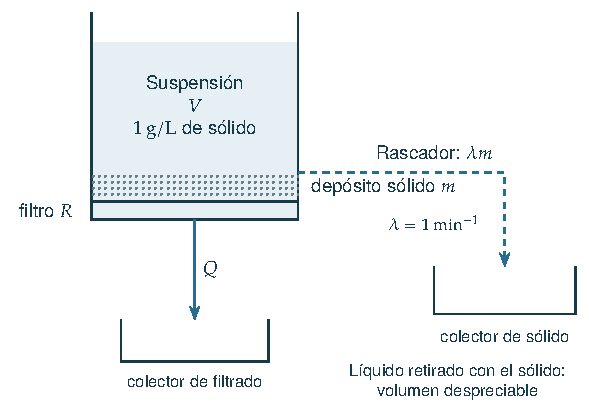
\includegraphics[width=11.17cm]{assets/M2-E0362-setup.pdf}\par
\smallskip{\small Rutas separadas del filtrado y del sólido retirado por el rascador.\par}
\end{minipage}
\end{center}
